\documentclass[fleqn,compress,utf8,aspectratio=169,t]{beamer}
% use LMU theme
\usetheme{LMU}

% This setups a lot of recommended settings and packages you usually need
% anyway. So let me take care for you and your document stays clear.

% Examples: Tables, Graphics, Listings, Hyperref...
%
% Prevent slide breaks in the middle of a paragraph
\widowpenalties 1 10000
\raggedbottom

\makeatletter
\@ifundefined{KOMAClassName}{% if non-KOMA class
  \IfFileExists{parskip.sty}{%
    \RequirePackage{parskip}
  }{% else
    \setlength{\parindent}{0pt}
    \setlength{\parskip}{6pt plus 2pt minus 1pt}}
}{% if KOMA class
  \KOMAoptions{parskip=half}}
\makeatother

\IfFileExists{xurl.sty}{\usepackage{xurl}}{} % add URL line breaks if available
\IfFileExists{bookmark.sty}{\usepackage{bookmark}}{\usepackage{hyperref}}
\urlstyle{same} % disable monospaced font for URLs

\usepackage{listings}
\lstset{defaultdialect=[5.3]Lua}
\lstset{defaultdialect=[x86masm]Assembler}
\usepackage{longtable,booktabs}
\usepackage{caption}
% Make caption package work with longtable
\makeatletter
\def\fnum@table{\tablename~\thetable}
\makeatother
\usepackage{graphicx}
\makeatletter
\def\maxwidth{\ifdim\Gin@nat@width>\linewidth\linewidth\else\Gin@nat@width\fi}
\def\maxheight{\ifdim\Gin@nat@height>\textheight\textheight\else\Gin@nat@height\fi}
\makeatother
% Scale images if necessary, so that they will not overflow the page
% margins by default, and it is still possible to overwrite the defaults
% using explicit options in \includegraphics[width, height, ...]{}
\setkeys{Gin}{width=\maxwidth,height=\maxheight,keepaspectratio}
% Set default figure placement to htbp
\makeatletter
\def\fps@figure{htbp}
\makeatother
\usepackage[normalem]{ulem}
% Avoid problems with \sout in headers with hyperref
\pdfstringdefDisableCommands{\renewcommand{\sout}{}}
\setlength{\emergencystretch}{3em} % prevent overfull lines
%Tightlist Command
\providecommand{\tightlist}{%
  \setlength{\itemsep}{0pt}\setlength{\parskip}{0pt}}



\usepackage[style=ieee]{biblatex}
\addbibresource{slides.bib}
\usepackage{multirow}

\usepackage{tikz} 
\usetikzlibrary{calc}
\newcommand{\AsymCloud}[3]{
\begin{scope}[shift={#1},scale=#3]
\draw (-1.6,-0.7) .. controls (-2.3,-1.1)
and (-2.7,0.3) .. (-1.7,0.3)coordinate(asy1) .. controls (-1.6,0.7)
and (-1.2,0.9) .. (-0.8,0.7) .. controls (-0.5,1.5)
and (0.6,1.3) .. (0.7,0.5) .. controls (1.5,0.4)
and (1.2,-1) .. (0.4,-0.6)coordinate(asy2) .. controls (0.2,-1)
and (-0.2,-1) .. (-0.5,-0.7) .. controls (-0.9,-1)
and (-1.3,-1) .. cycle;
\node (cloud) at (-0.5,0.5) {#2};
\end{scope}
}

%%%%%%%%%%%%%%%%%%%%%%%%%%%%%%%%%%%%%%%%%%%%%%%%%%%%%%%%%%%%%%%%%%%%%%%%%%%%%%%%
%%                                 Customizations                             %%
%%%%%%%%%%%%%%%%%%%%%%%%%%%%%%%%%%%%%%%%%%%%%%%%%%%%%%%%%%%%%%%%%%%%%%%%%%%%%%%%

% If you want no navigation uncomment this
%\beamertemplatenavigationsymbolsempty

% setup listings
\lstset{
  basicstyle=\ttfamily\color{black},
  showstringspaces=false
}

\lstdefinestyle{highlight}{
  keywordstyle=\color{red},
  commentstyle=\color{lmu@darkgray}
}

\lstdefinestyle{basetex}{
language={[LaTeX]Tex},
basicstyle=\color{black!40},
keywordstyle=\color{red!40},
commentstyle=\color{lmu@darkgray!40},
moredelim=**[il][\only<+>{\color{black}\lstset{style=highlight}}]{@}
}

\lstdefinestyle{basec}{
language=C,
basicstyle=\color{black!40},
keywordstyle=\color{red!40},
commentstyle=\color{green!40},
moredelim=**[il][\only<+>{\color{black}\lstset{style=highlight}}]{@}
}

%%%%%%%%%%%%%%%%%%%%%%%%%%%%%%%%%%%%%%%%%%%%%%%%%%%%%%%%%%%%%%%%%%%%%%%%%%%%%%%%
%%                                  Title Page Data                           %%
%%%%%%%%%%%%%%%%%%%%%%%%%%%%%%%%%%%%%%%%%%%%%%%%%%%%%%%%%%%%%%%%%
% helper command to add multiple authors
\newcommand{\newauthor}[2]{
\parbox[c]{0.26\textwidth}{
{\bfseries #1} \\
{\scriptsize{\href{mailto:#2}{#2}}}
}
%{#1}
}

% Authors
\author[Lösch]{
  \newauthor{Robin Lösch}{loesch@cip.ifi.lmu.de}
}

\institute[LMU]{
  {MNM-Team, LMU München}
}

\date[\today]{\today}

\title{Towards Quantum-Resistant MACSec using EAP-TLS}
\subtitle{Abschlussvortrag zur Masterarbeit}

\hypersetup{
  pdftitle={Title},
  pdfauthor={Author},
  hidelinks}


%%%%%%%%%%%%%%%%%%%%%%%%%%%%%%%%%%%%%%%%%%%%%%%%%%%%%%%%%%%%%%%%%%%%%%%%%%%%%%%%
%%                                  Document                                  %%
%%%%%%%%%%%%%%%%%%%%%%%%%%%%%%%%%%%%%%%%%%%%%%%%%%%%%%%%%%%%%%%%%%%%%%%%%%%%%%%%

\begin{document}

\begin{frame}
  \titlepage
\end{frame}

%%%%%%%%%%%%%%%%%%%%%%%%%%%%%%%%%%% Overview %%%%%%%%%%%%%%%%%%%%%%%%%%%%%%%%%%%

\section{The QuaSiModO Project}

\begin{frame}{}
  \vspace{0cm}
  \centering
  \begin{tikzpicture}
    \node[inner sep=0pt] (8021x) at (0,0)
        {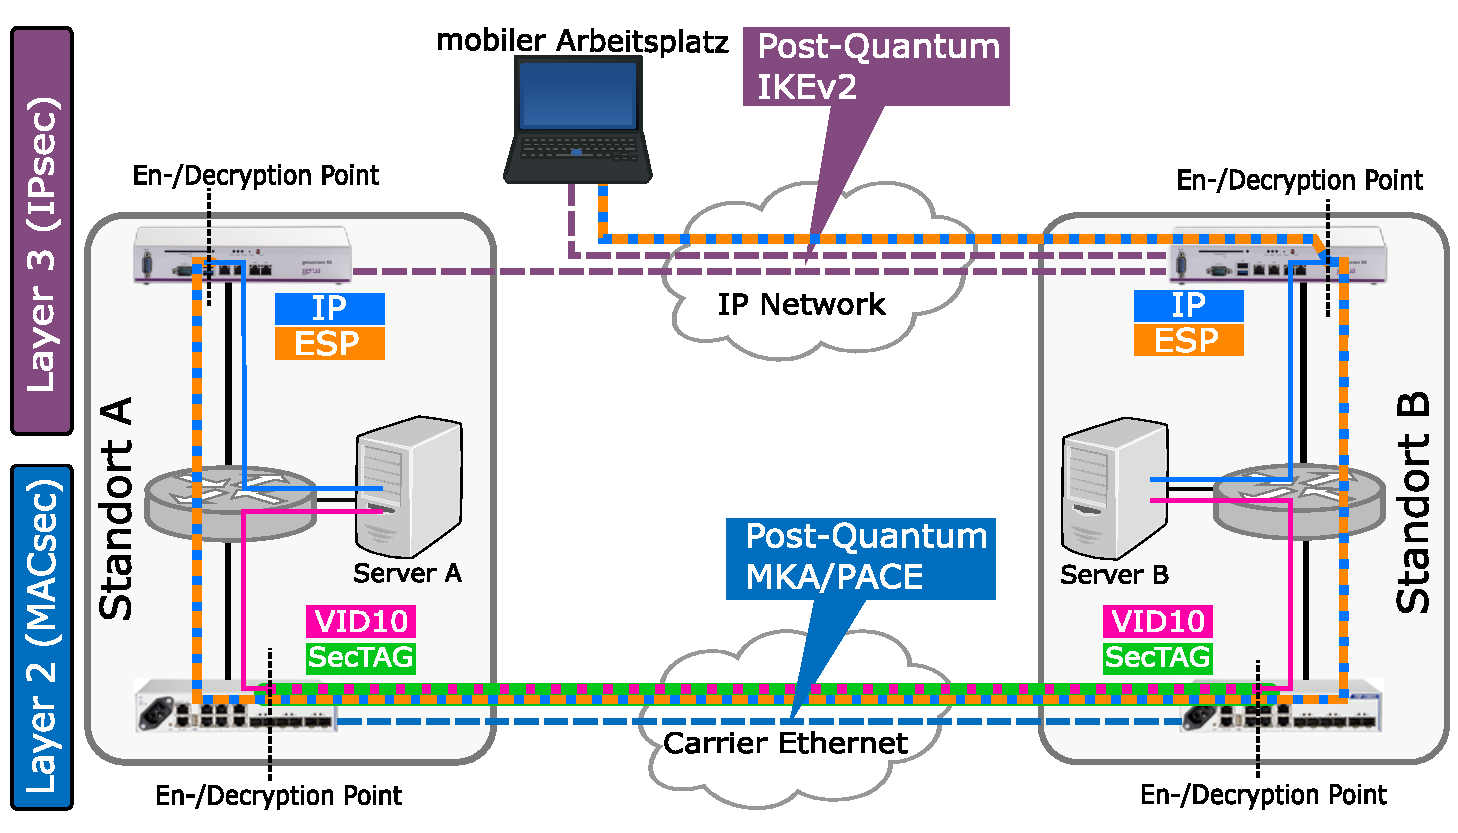
\includegraphics[width=0.8\textwidth]{konzept-quasi_2.pdf}};
        \draw<2> [line width=0.25mm,draw=red] (-5.6,-0.2) rectangle (5.6,3.1);
        \draw<3> [line width=0.25mm,draw=red] (-5.6,-3.1) rectangle (5.6,-0.2);
    \end{tikzpicture}
\end{frame} 
\section{Background \& Motivation}

\subsection{MACSec}

\begin{frame}{MACSec}
  \begin{itemize}
    \item IEEE Standard
    \item Layer 2 encryption \& integrity protection 
    \item<2-> Two important standards:
    \begin{itemize}
      \item IEEE 802.1X: Port-Based Network Access Control\cite{IEEE8021X}
      \item IEEE 802.1AE: Media Access Control (MAC) Security\cite{IEEE8021AE}
    \end{itemize}
  \end{itemize}
\end{frame}

\begin{frame}{}
  \vspace{0.5cm}
  \begin{tikzpicture}
    \node[inner sep=0pt] (8021x) at (0,0)
        {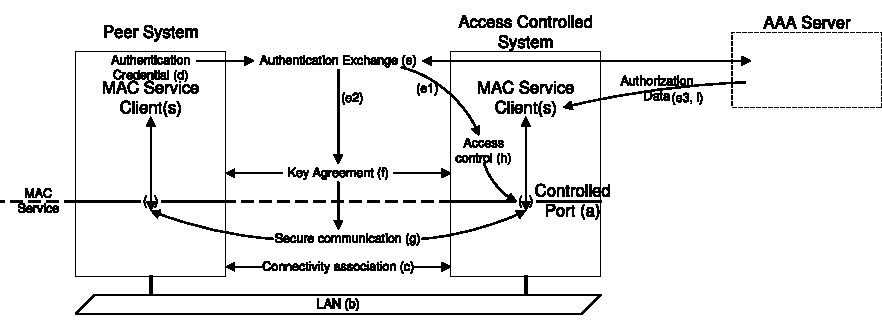
\includegraphics[width=1\textwidth]{8021x_fig_6_1_overview_2.pdf}};
        \draw<2> [line width=0.25mm,draw=red] (-6,-2) rectangle (-3,2.3);
        \draw<3> [line width=0.25mm,draw=red] (3,-2.5) rectangle (-6,-1.9);
        \draw<4> [line width=0.25mm,draw=red] (0,-2) rectangle (2.8,2.4);
        \draw<5> [line width=0.25mm,draw=red] (4.5,0.8) rectangle (7.3,2.4);
        \draw<6> [line width=0.25mm,draw=red] (-3.2,-0.5) rectangle (-0.1,2);
        \node<6> [line width=0.25mm,draw=none,text=red] at (-1.6,2.2) {EAP};
    \end{tikzpicture} 
\end{frame} 


\begin{frame}{Extensible Authentication Protocol\cite{rfc3748}}
  \begin{columns}[T]
    \column{0.9\textwidth}
  \begin{itemize}
    \item Framework for arbitrary authentication methods
    \item Request-Response based protocol
    \item<2-> IEEE 802.1X uses EAP-TLS
    \begin{itemize}
      \item TLS encapsulated in EAP
      \item (EC)DH and RSA for authentication and key exchange
    \end{itemize}
    \item<3-> Result:
    \begin{itemize}
      \item Mutual authentication (Access control)
      \item Shared symmetric key (MACSec encryption)
    \end{itemize}
  \end{itemize}
  \column{0.1\textwidth}
\end{columns}
\end{frame}

\iffalse
\begin{frame}{IEEE 802.1X (Port-Security)}
  \begin{columns}[T]
    \column{.5\textwidth}
  \begin{itemize}
    \item Mutual authentication in LANs
    \begin{itemize}
      \item<2-> Supplicant (Peer)\\
      Endpoints (Computer, Telephone, ...)
      \item<3-> Authenticator\\
      Network equipment (Router, Switch)
      \item<4-> Authentication Server\\
      AAA-Server (Radius, Diameter)
    \end{itemize}
  \item<5-> Authentication:
  \begin{itemize}
    \item Pre-shared Keys (Point-to-Point)
    \item EAP(-TLS)
  \end{itemize}
  \item<6-> Result: Connectivity association
\end{itemize}
\column{.6\textwidth}
\begin{figure}[t]
  \centering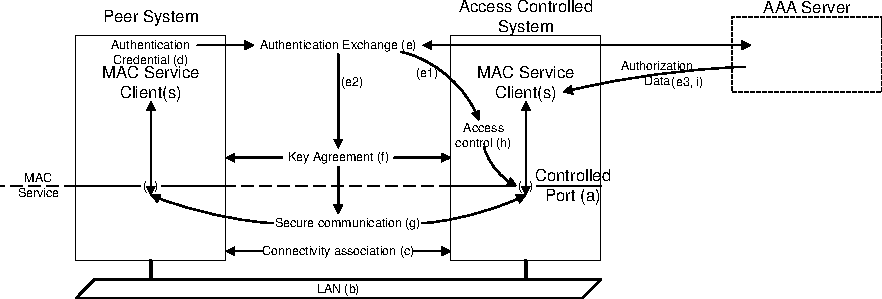
\includegraphics[trim={0 0 0 0}, clip, width=1.0\columnwidth]{8021x_fig_6_1_overview.pdf}
\end{figure}
\end{columns}
\end{frame}

\begin{frame}{IEEE 802.1AE (MACSec)}
  \begin{columns}[T]
    \column{.6\textwidth}
    \begin{itemize}
      \item Connectivity Association\\
      Between Peer and Authenticator
      \item<2-> MKA Protocol \\
      Mutual "Secure Channel" between Peers
      \item<3-> Secure Channel $\equiv$ Shared symmetric key
      \item<4-> Enables secured frames
      \begin{itemize}
        \item Confidentiality (Encryption)\\
        \item Integrity Protection (MAC)
      \end{itemize}
    \end{itemize}
  \column{.5\textwidth}
      \begin{figure}[t]
        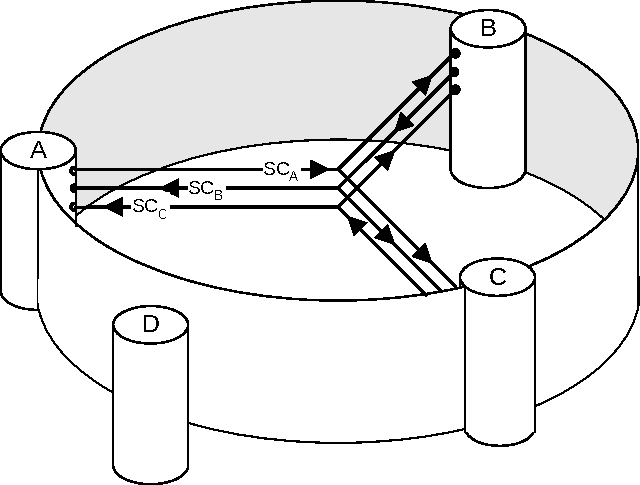
\includegraphics[trim={0 0 0 2}, width=1\columnwidth]{8021ae_fig_7_6_ca.pdf}
    \end{figure}
  \end{columns}
\end{frame}
\fi

\subsection{Post-Quantum Cryptography}

\begin{frame}{Post-Quantum Cryptography}
  \begin{columns}[T]
    \column{0.9\textwidth}
  \begin{itemize}
    \item Quantum computers are an inherent problem for asymmetric cryptography
    \item<2-> Alternative cryptosystems have been researched for years:
    \begin{itemize}
      \item McEliece (1978): Code-based cryptosystems\cite{berlekamp1978inherent}
      \item Lamport (1979): Hash-based signatures\cite{lamport1979constructing}
      \item Imai, Matsumoto (1988): Multivariate cryptography\cite{matsumoto1988public}
      \item Ajtai (1996): Lattice-based cryptosystems\cite{ajtai1996generating}
      \item De Feo, Jao, and Plût (2011): (Supersingular) Isogeny-based DH\cite{jao2011towards}
    \end{itemize}
    \item<3-> NIST standardization project: One or more PQ cryptosystems
    \item<4-> Which cryptosystem is a good replacement for DH, RSA...?
  \end{itemize}
  \column{0.1\textwidth}
\end{columns}
\end{frame}

\iffalse
\begin{frame}{Cryptography used in MACSec}
  \begin{columns}[T]
    \column{0.9\textwidth}
  \begin{itemize}
    \item<2-> IEEE 802.1AE
    \begin{itemize}
      \item Solely relies on symmetric ciphers
      \item Simple solution: Doubled key space
    \end{itemize}
    \item<3-> IEEE 802.1X
    \begin{itemize}
      \item Authentication (Asymmetric Signatures)
      \item Key Exchange (Asymmetric Encryption)
    \end{itemize}
  \end{itemize}
  \column{0.1\textwidth}
\end{columns}
\end{frame}
\fi
\begin{frame}{Finding a good replacement}
  \begin{columns}[T]
    \column{0.5\textwidth}
  \begin{itemize}
    \item Main focus of this work
    \item<2-> There is no clear "winner"
    \item<3-> Different requirements/different trade-offs
    \begin{itemize}
      \item Small key sizes (traffic footprints)
      \item Fast algorithms (latency) 
      \item ``Maturity''
    \end{itemize}
  \end{itemize}
  \column{0.5\textwidth}
  \vspace*{-0.5cm}
  \begin{figure}[t]
    \includegraphics<3->[width=1\columnwidth]{plot_scatter_all_latency_pubkeysize.pdf}
  \end{figure}
\end{columns}
\end{frame}

\iffalse
\begin{frame}{Problem Statement}
  \begin{columns}[T]
  \column{.45\textwidth}
    \begin{itemize}
      \item IEEE 802.1AE relies on 802.1X
      \item<2-> IEEE 802.1X relies on EAP-TLS
      \item<3-> EAP-TLS uses weak algorithms
      \item<4-> No obvious replacement
    \end{itemize}
  \column{.55\textwidth}
  \vspace*{-1cm}
    \begin{figure}[t]
      \includegraphics<4>[width=1\columnwidth]{plot_scatter_all_latency_pubkeysize.pdf}
      \includegraphics<5->[width=1\columnwidth]{plot_scatter_all_latency_pubkeysize_sign.pdf}
    \end{figure}
  \end{columns}
\end{frame}
\fi

\section{Requirements}

\begin{frame}{Requirements for a PQ MACSec}
  \begin{columns}[T]
    \column{0.9\textwidth}
    \begin{itemize}
      \item Main Goals:
      \begin{itemize}
        \item Quantum-resistant design
        \item Keep existing security properties
      \end{itemize}
      \item<2-> Key Exchange Algorithm / Signature Algorithms:
      \begin{itemize}
        \item Latency > Traffic
        \item Forward-secrecy for Key Exchange
      \end{itemize}
      \item<3-> Need to evaluate different algorithms
    \end{itemize}
    \column{0.1\textwidth}
  \end{columns}
\end{frame}

\section{Design/Evaluation}

\begin{frame}{Methodology}
  \begin{columns}[T]
    \column{0.9\textwidth}
    \begin{itemize}
      \item<2-> Implement PQ MACSec:
      \begin{itemize}
        \item hostapd (Peer/Access Controlled System)
        \item FreeRADIUS (Authentication Server)
        \item OpenSSL fork by Open Quantum Safe
      \end{itemize}
      \item<3-> Experimental evaluation of all NIST Round 3 candidates
      \item<4-> Practical proof-of-concept
    \end{itemize}
  \column{0.1\textwidth}
\end{columns}
\end{frame}

\section{Results}

\begin{frame}{Performance Evaluation}
  \begin{columns}[T]
    \column{.5\textwidth}
      \begin{itemize}
        \item Strongly depends on foundation
        \item<2-> Performance often similar to ECDH
      \end{itemize}
      \vspace{10px}
      \tiny
      \only<2>{
      \begin{table}
        \begin{tabular}{llc}
                \hline
                \textbf{Foundation} & \textbf{Scheme} \\
                \hline
                \multirow{3}{*}{Code-Based} 
                & BIKE  \\
                & Classic McEliece \\
                & HQC \\
                \hline
                \multirow{5}{*}{Lattice-Based} 
                & SABER \\
                & CRYSTALS-KYBER \\
                & NTRU \\
                & NTRU Prime  \\
                & FrodoKEM \\
                \hline
                Isogeny-Based & SIKE \\
                \hline
            \end{tabular}
        \label{table:nist_round_2_kem}
    \end{table}}
    \only<3>{
      \begin{table}
        \begin{tabular}{llc}
                \hline
                \textbf{Foundation} & \textbf{Scheme} \\
                \hline
                \multirow{2}{*}{Lattice-Based} 
                & CRYSTALS-DILITHIUM \\
                & FALCON \\
                \hline
                \multirow{2}{*}{Multivariate} 
                    & GeMSS \\
                    & Rainbow  \\
                \hline
                Zero-Knowledge Proof & Picnic  \\
                \hline
                Hash-Based & SPHINCS+  \\
                \hline
            \end{tabular}
        \label{table:nist_round_2_dss}
    \end{table}
    
    }
    \column{.5\textwidth}
      \vspace*{-0.5cm}
      \begin{figure}
        \includegraphics<2>[trim={0 0 0 0}, width=1\columnwidth]{plot_box_total_runtime.pdf}
        \includegraphics<3->[trim={0 0 0 0}, width=1\columnwidth]{plot_box_total_runtime_sig.pdf}
      \end{figure}
    \end{columns}
\end{frame}

\begin{frame}{Impact of Latency}
  \begin{columns}[T]
    \column{.4\textwidth}
      \begin{itemize}
        \item Large number of frames
        \item EAP Packets need to be acknowledged
        \item Wall-Clock Runtime strongly depends on latency
      \end{itemize}
    \column{.6\textwidth}
      \vspace*{-0.5cm}
      \begin{figure}[t]
        \centering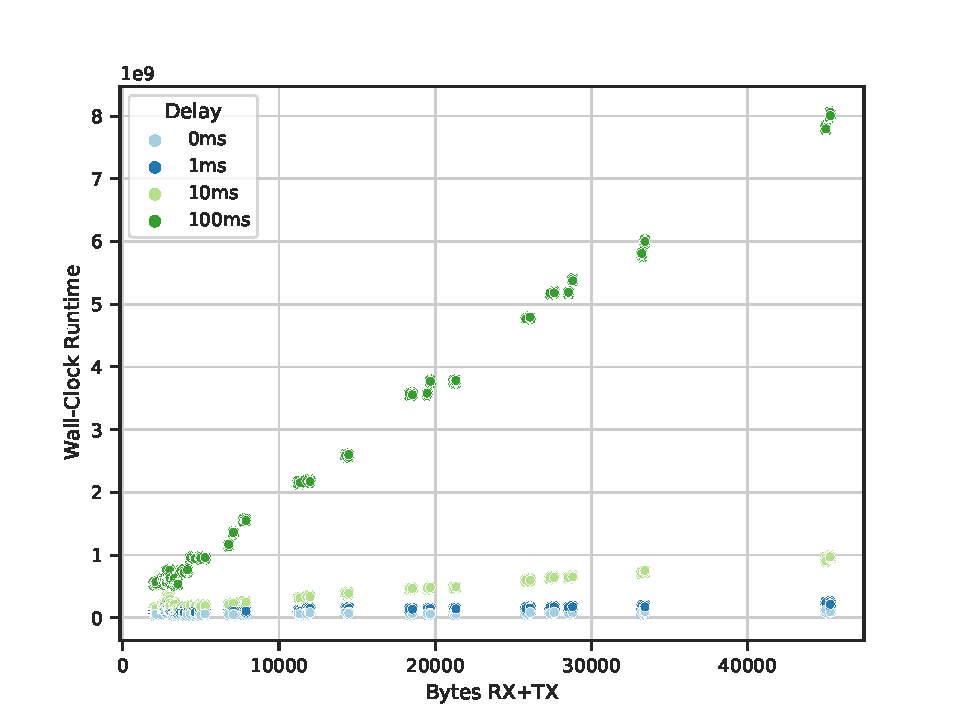
\includegraphics[trim={-10px 0 0 0}, clip, width=1\columnwidth]{plot_scatter_handshake_time_vs_traffic_delay.pdf}
      \end{figure}
    \end{columns}
\end{frame}

\begin{frame}{Forward-secrecy}
  \begin{columns}[T]
    \column{.4\textwidth}
      \begin{itemize}
        \item Forward-secrecy by design
        \begin{itemize}
          \item NIST uses Three-way API
          \item Generate, Encapsulate, Decapsulate
        \end{itemize}
        \item Little impact on most algorithms
        \item Exception: SIDH/SIKE
      \end{itemize}
    \column{.6\textwidth}
      \vspace*{-0.5cm}
      \begin{figure}[t]
        \centering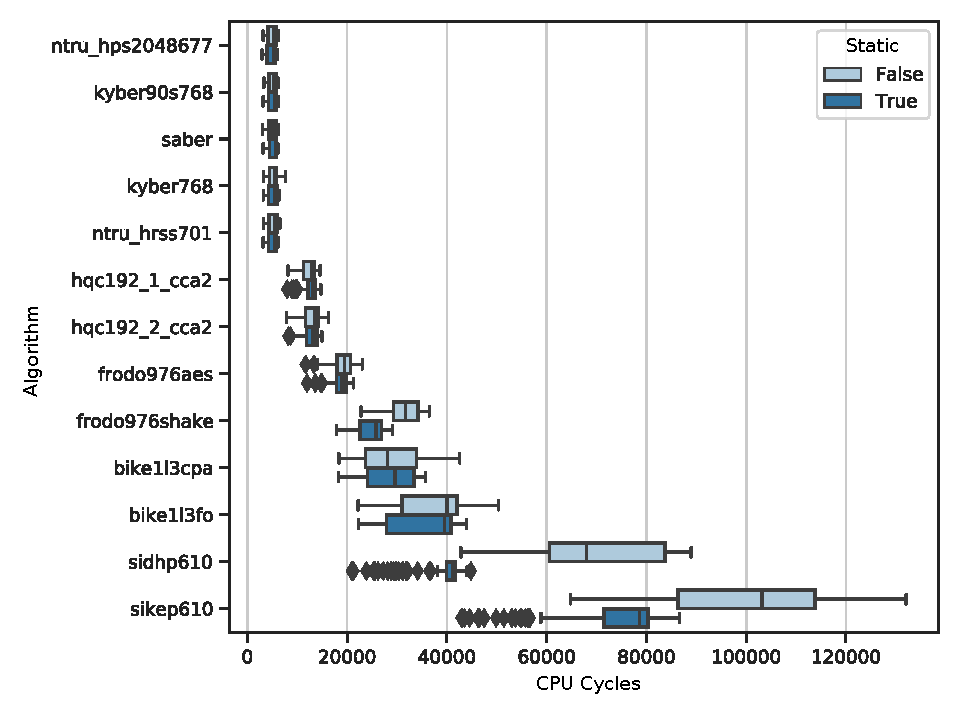
\includegraphics[trim={-10px 0 0 0}, clip, width=1\columnwidth]{plot_box_static.pdf}
      \end{figure}
    \end{columns}
\end{frame}

\begin{frame}{Practical Evaluation}
  \begin{columns}[T]
    \column{.6\textwidth}
      \begin{itemize}
        \item Part of QuaSiModO
        \item Cooperation with ADVA Optical Networking
        \item Selected PQ schemes compared to classical schemes
      \end{itemize}
      \vspace{5mm}
      \scriptsize
        \begin{table}[h]
          \begin{center}
              \begin{tabular}{lrrr}
                  \hline
              \textbf{Setting} & \textbf{Signature} & \textbf{KEX} \\
              \hline
              PQ & falcon1024 & Saber \\
              \hline
              ECDH & P-521 & P-384 \\
              \hline
              Hybrid & falcon1024 \(\vert\vert\) P-521 & Saber \(\vert\vert\) P-384  \\
              \hline
              RSA & RSA4096 & P-384 \\
              \hline
              \end{tabular}
              \label{table:pubkeysizes_practical}
          \end{center}
      \end{table}
    \column{.5\textwidth}
    \vspace*{-0.5cm}
    \only<1-2>{
      \begin{figure}
        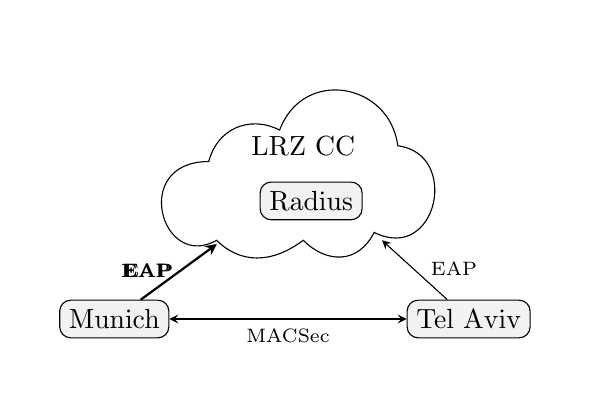
\begin{tikzpicture}
          \useasboundingbox [fill=none] (-4cm,-2.3cm) rectangle (3,2);
          \tikzstyle{box} = [rectangle, rounded corners, text centered, draw=black, fill=gray!10]
          \tikzstyle{arrow} = [->,>=stealth]
          \tikzstyle{arrowthick} = [thick,->,>=stealth]
          \tikzstyle{doublearrow} = [<->,>=stealth]
          \color{white}
          \color{black!75!black}
          \node (a) [box, yshift=-0.2cm, xshift=-0.4cm] {Radius};
          \node (b) [box, below of=a, yshift=-0.5cm, xshift=-2.5cm] {Munich};
          \node (c) [box, right of=b, xshift=3.5cm] {Tel Aviv};
          \draw [arrow] (b) -- node[above, xshift=-.4cm, yshift=-.2cm] {\scriptsize EAP} (-1.6,-0.75);
          \draw<2-> [arrowthick] (b) -- node[above, xshift=-.4cm, yshift=-.2cm] {\scriptsize \textbf{EAP}} (-1.6,-0.75);
          \draw [arrow] (c) -- node[above, xshift=.5cm, yshift=-.2cm] {\scriptsize EAP} (0.5,-0.7);
          \draw [doublearrow] (b) -- node[below] {\scriptsize MACSec} (c);
          \AsymCloud{(0,0)}{LRZ CC}{1}
        \end{tikzpicture} 
      \end{figure}}
      \onslide<3->{
      \begin{figure}[t]
        \centering\includegraphics<3->[trim={0 0 0 0}, clip, width=1\columnwidth]{plot_scatter_practical.pdf}
      \end{figure}}
    \end{columns}
\end{frame}

\section{Summary}

%\begin{frame}{Contribution}
%  \small
%      \begin{itemize}
%        \item Design and Implementation of PQ IEEE802.1X/EAP-TLS
%        \item PQ and TLS1.3 for hostapd/FreeRADIUS
%        \begin{itemize}
%          \scriptsize
%          \item \url{https://github.com/crest42/freeradius-server}
%          \item \url{https://github.com/crest42/hostapd}
%        \end{itemize}
%        \item Contributions for liboqs/OpenSSL
%        \begin{itemize}
%          \scriptsize
%          \item \url{https://github.com/open-quantum-safe/openssl/pull/239}
%          \item \url{https://github.com/open-quantum-safe/openssl/pull/257}
%        \end{itemize}
%        \item Extensive Evaluation of different algorithms
%        \item Proof-of-Concept on a practical implementation
%      \end{itemize}
%\end{frame}

\begin{frame}{}
  \small
  \begin{columns}[T]
    \column{.5\textwidth}
      \begin{itemize}
        \item[]<2-> \textbf{Conclusion}
        \begin{itemize}
          \scriptsize
          \item PQ Crypto is feasible
          \item Biggest concern are key sizes
          \item Lattice-based ciphers performs best
          \item EAP/Radius are bottlenecks
        \end{itemize}
      \end{itemize}
    \column{.5\textwidth}
    \begin{itemize}
      \item[]<3-> \textbf{Contribution}
      \begin{itemize}
        \scriptsize
        \item PQ IEEE802.1X/EAP-TLS
        \item PQ TLS1.3 implementation of hostapd/FreeRADIUS
        \item Contributions for liboqs/OpenSSL
        \item Extensive evaluation
        \item Real-World proof-of-concept
      \end{itemize}
    \end{itemize}
    
    \end{columns}
    \begin{columns}[b]
      \begin{column}{0.3\textwidth}
      \end{column}
      \begin{column}{0.5\textwidth}
        \begin{center}
          \begin{itemize}
            \item[]<4-> \textbf{Future Work}
            \begin{itemize}
              \scriptsize
              \item TEAP instead of EAP-TLS
              \item (PQ-)TLS 1.4?
              \item Further NIST project development
            \end{itemize}
          \end{itemize}
      \end{center}
    \end{column}
    \begin{column}{0.2\textwidth}

    \end{column}
  \end{columns}
\end{frame}

\section{Appendix}
\begin{frame}[noframenumbering,allowframebreaks]
  \frametitle{References}
  \nocite{*}
  \printbibliography[heading=none]
\end{frame}

\begin{frame}[noframenumbering]{Traffic Evaluation}
  \begin{columns}[T]
    \column{.6\textwidth}
      \begin{itemize}
        \item Algo. selection depends heavily on use-case
        \item Small keys vs. small signatures
      \end{itemize}
      \vspace{10px}
      \tiny
      \only<2->{
      \begin{table}
        \begin{tabular}{llc}
                \hline
                \textbf{Background} & \textbf{Scheme} \\
                \hline
                \multirow{3}{*}{Code-Based} 
                & BIKE  \\
                & Classic McEliece \\
                & HQC \\
                \hline
                \multirow{5}{*}{Lattice-Based} 
                & SABER \\
                & CRYSTALS-KYBER \\
                & NTRU \\
                & NTRU Prime  \\
                & FrodoKEM \\
                \hline
                Isogeny-Based & SIKE \\
                \hline
            \end{tabular}
        \label{table:nist_round_2_kem}
    \end{table}}
   
      \column{.5\textwidth}
      \vspace*{-1cm}
      \begin{figure}
        \includegraphics<2->[trim={0 0 0 0}, width=1\columnwidth]{plot_bar_traffic2.pdf}
      \end{figure}
    \end{columns}
\end{frame}

\begin{frame}[noframenumbering]{Protocol Overhead}
  \begin{columns}[T]
    \column{.6\textwidth}
      \begin{itemize}
        \item Many protocol layers
        \item Results in large overhead
        \item<3-> Redundant AVP values
        \item<3-> Sparse variant can save up to \(40\%\)
      \end{itemize}
      \column{.5\textwidth}
      \vspace*{-1cm}
      \begin{figure}
        \includegraphics<2>[trim={0 0 0 0}, width=1\columnwidth]{plot_avp.pdf}
        \includegraphics<3->[trim={0 0 0 0}, width=1\columnwidth]{plot_avp_sparse.pdf}
      \end{figure}
    \end{columns}
\end{frame}

\begin{frame}[noframenumbering]{Post-Quantum Cryptography}
  \begin{columns}[T]
    \column{.8\textwidth}
      \begin{itemize}
        \item<2-> 40 Years of quantum computing:
        \begin{itemize}
          \item 1980: First (theoretical) model of a quantum turing machine
          \item 2018: 72-Qubit ``Bristlecone'' architecture
        \end{itemize}
        \item<3-> Quantum-effects allow for faster algorithms:
              \begin{itemize}
                \item Shor's algorithm: Breaks RSA and (EC)DH in polynomial time
                \item Grover's algorithm: Weaken symmetric schemes by $\sqrt{n}$
              \end{itemize}
        \item<4-> When will quantum computer be able to break RSA2048?
      \end{itemize}
      \vfill
  \column{.2\textwidth}
  \begin{figure}[t]
    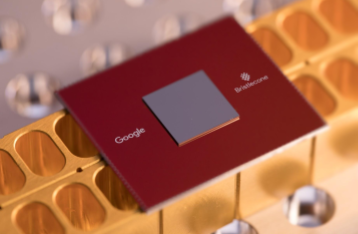
\includegraphics[width=1\columnwidth]{bristlecone.png}
  \end{figure}
  \end{columns}
\end{frame}

\begin{frame}[noframenumbering]{Fragment Size}
  \begin{figure}[t]
    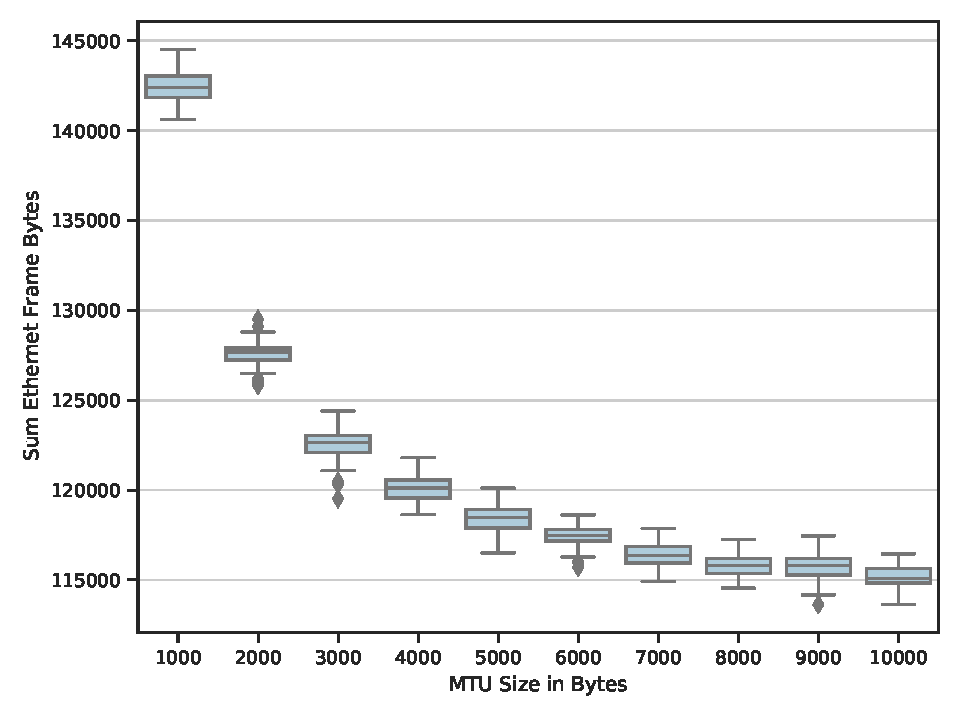
\includegraphics[width=0.5\textwidth]{plot_box_fragment_size.pdf}
  \end{figure}
\end{frame}

\begin{frame}[noframenumbering]{Shor}
  \begin{figure}[t]
    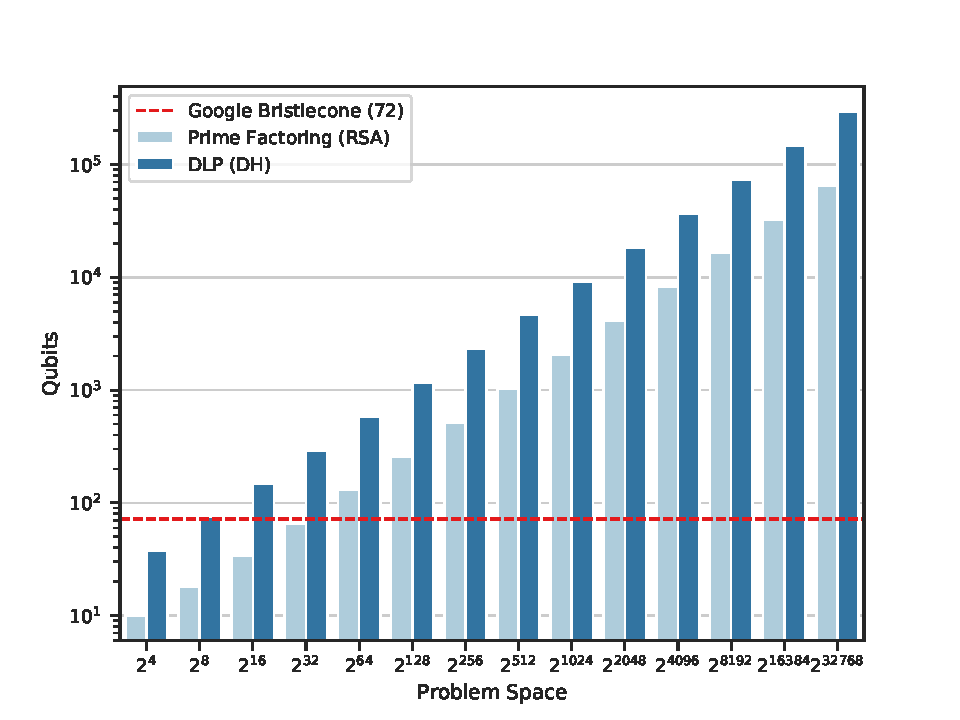
\includegraphics[width=0.5\textwidth]{plot_line_shor_rsa.pdf}
  \end{figure}
\end{frame}



\end{document}
